\documentclass[conference]{IEEEtran}
\IEEEoverridecommandlockouts
% The preceding line is only needed to identify funding in the first footnote. If that is unneeded, please comment it out.
\usepackage{cite}
\usepackage{amsmath,amssymb,amsfonts}
\usepackage{algorithmic}
\usepackage{graphicx}
\usepackage{textcomp}
\usepackage{xcolor}
\def\BibTeX{{\rm B\kern-.05em{\sc i\kern-.025em b}\kern-.08em
    T\kern-.1667em\lower.7ex\hbox{E}\kern-.125emX}}
\begin{document}

\title{Edge computing testbed for V2I applications prototyping and evaluation *\\
{\footnotesize \textsuperscript{*}Note: Sub-titles are not captured in Xplore and
should not be used}
\thanks{funded by AT}
}

\author{\IEEEauthorblockN{1\textsuperscript{st} Zeinab Nezami}
\IEEEauthorblockA{\textit{School of Computing} \\
\textit{University of Leeds}\\
Leeds, United Kingdom \\
email address or ORCID}
\and
\IEEEauthorblockN{2\textsuperscript{nd} Evangelos Pournaras}
\IEEEauthorblockA{\textit{School of Computing} \\
\textit{University of Leeds}\\
Leeds, United Kingdom \\
email address or ORCID}
\and
\IEEEauthorblockN{6\textsuperscript{th} Given Name Surname}
\IEEEauthorblockA{\textit{dept. name of organization (of Aff.)} \\
\textit{name of organization (of Aff.)}\\
City, Country \\
email address or ORCID}
}

\maketitle

\begin{abstract}

\end{abstract}

\begin{IEEEkeywords}
Edge Computing, V2I application, Testbed 
\end{IEEEkeywords}

\section{Introduction}

Challenges: 
ITS applications should deal with various data provided
through various communication links. The density and the
mobility of the vehicles are the major factors to take into account
when developing V2X applications that are destined to run in
mobile edge computing distributed environment. In a high-density
scenario, the application must use the available bandwidth
efficiently in order to deliver its service continuously to the
subscribed nodes. The application should also deal with nodes
joining/leaving the network during their mouvement and
guarantee the service continuity. The MEC infrastructure is
intended to offer a management system and a couple of standard
services that facilitate the aforementioned properties. The MEC
infrastructure introduces a whole new service model that requires
an adapted development paradigm.
An important aspect that should be taken into account while
developing a V2X application that targets MEC as a deployment
environment is to ensure the proper interaction of the application
with the management entities and the system components. At the
development phase of a V2X MEC service components testing in
real environment increase deployment time, costs, and
complexity. In the next section, we analyze the standard
deployment architecture proposed by the European
Telecommunications Standards Institute (ETSI) to extract the
main components and their functionalities.

\section{Related work}
\begin{table}[htbp]
\caption{Table Type Styles}
\begin{center}
\begin{tabular}{|c|c|c|c|}
\hline
\textbf{Table}&\multicolumn{3}{|c|}{\textbf{Table Column Head}} \\
\cline{2-4} 
\textbf{Head} & \textbf{\textit{Table column subhead}}& \textbf{\textit{Subhead}}& \textbf{\textit{Subhead}} \\
\hline
copy& More table copy$^{\mathrm{a}}$& &  \\
\hline
\multicolumn{4}{l}{$^{\mathrm{a}}$Sample of a Table footnote.}
\end{tabular}
\label{tab1}
\end{center}
\end{table}


\section{Testbed Design}
\par The proposed testbed aims at helping researchers and developers to design and verify distributed
V2I applications and algorithms destined to run in an edge computing environment. 
The main components of the testbed are agent, network infrastructure, service distributor, connector, and system orchestrator. The following subsections outline the modules as shown in Fig.\ref{fig:model}.
\begin{figure}[!htbp]
\centering
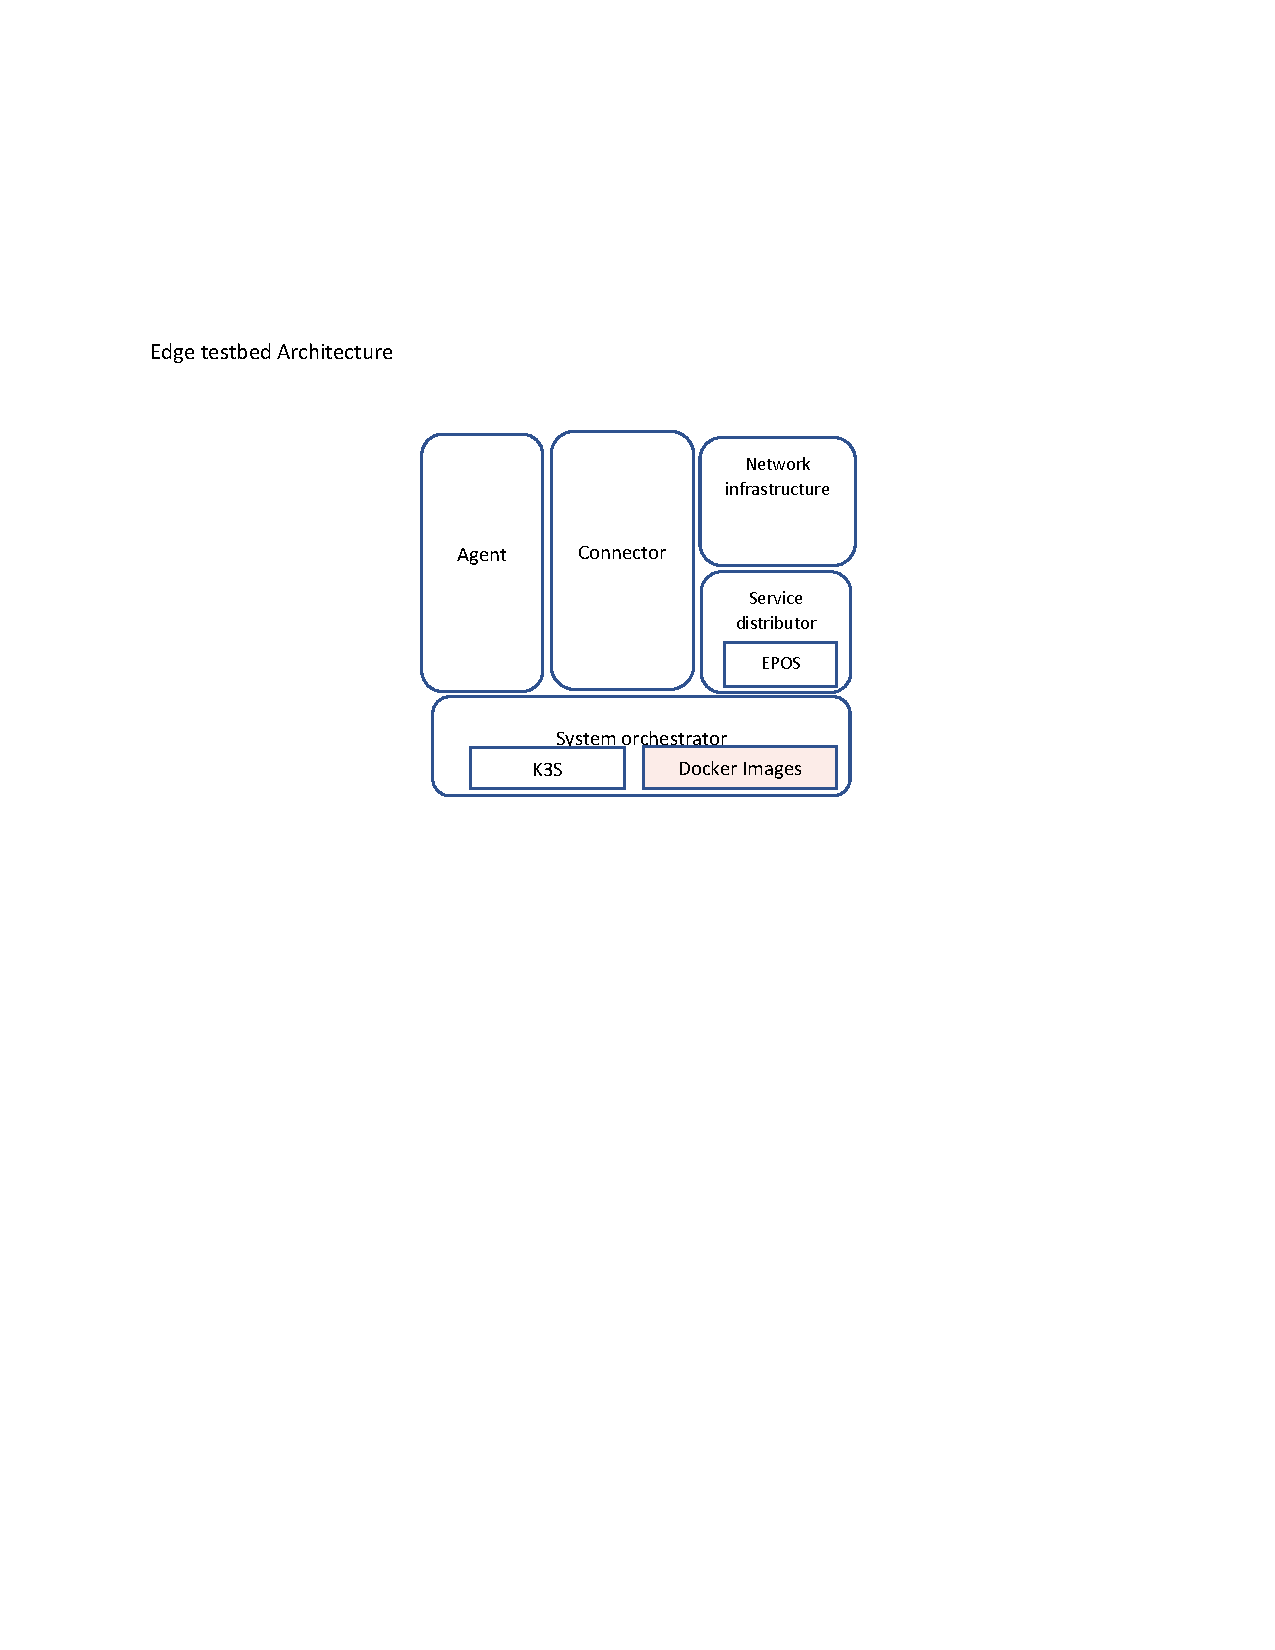
\includegraphics[clip, trim=6cm 14.0cm 6.0cm 6.5cm, width=\columnwidth]{figures/model1.pdf}
\caption{Proposed test-bed model}
\label{fig:model}
\end{figure}

\subsection{Agent}
\par An agent is an abstraction of a mobile entity such as vehicle or mobile device equipped with a set of sensors (e.g., GPS, camera), enabling the surrounding environment perception (e.g., position, speed, temperature) and a set of actuators (e.g., display, acceleration). 
\subsubsection{Mobility module}
\par Each agent has a mobility profile. This module's tasks consist of initiating/updating vehicle nodes position, creating/destroying communication's links, and managing mobility
The mobility support is achieved through the use of the mobile nodes’ positions regarding the fixed edge nodes and the city map to create and destroy communication links in runtime.
\subsection{Network infrastructure}
\par The edge infrastructure offers a distributed limited storage and processing capabilities in the vicinity of the agents to cope with the Cloud issues in running V2I applications regarding real-time services ultra-low latency requirements.
Edge computing offers ultra-low latency, high bandwidth, and real-time access to radio network information that can be leveraged by emerging vehicular safety and navigating applications. The "edge node" term refers to the combination of base stations (or access points) and edge servers close to the mobile radio network. 
 \subsection{Connector} 
\par Cellular networks are characterized by a wide communication range, which allows a base station to maintain connectivity with a network agent (vehicle) as long as possible, which means fewer handover operations. The upcoming Fifth Generation cellular network (5G) is one of the leading technologies that promises to grant a very high network capacity that guarantees high throughput/bandwidth for demanding applications like Augmented reality on autonomous vehicles. 5G networks will natively include mobile edge computing capabilities by design that may support different vehicular communication technologies. In our testbed, connector is responsible for connecting different entities together and synchronising data pipelines. The communication of vehicles with a serving entity through a network is also managed with the connector.
\subsection{System orchestrator}
\par The management layer named orchestrator maintains an overall view on available computing, storage, and networking resources and services. It is responsible for:
\begin{itemize}
\item Scaling up and down the available resources as required by the running applications. 
\item Allocating and releasing the storage, networking, and compute resources offered by the service distributor.
\item Storing application images for faster instantiation procedure when it is required.
\item Providing support for fault and performance monitoring by collecting resources and running application
data and transmitting them to evaluation entities(?).
\end{itemize}
\subsection{Service distributor}
\par It handles the task of the appropriate host selection for requested services deployment by taking into account the application requirements, the available resources, and the network nodes' positions.

\section{Architecture/implementation}
\par The general architecture and the essential components of our proposed testbed are illustrated
in Fig.\ref{fig:arch} 

\begin{figure}[!htbp]
\centering
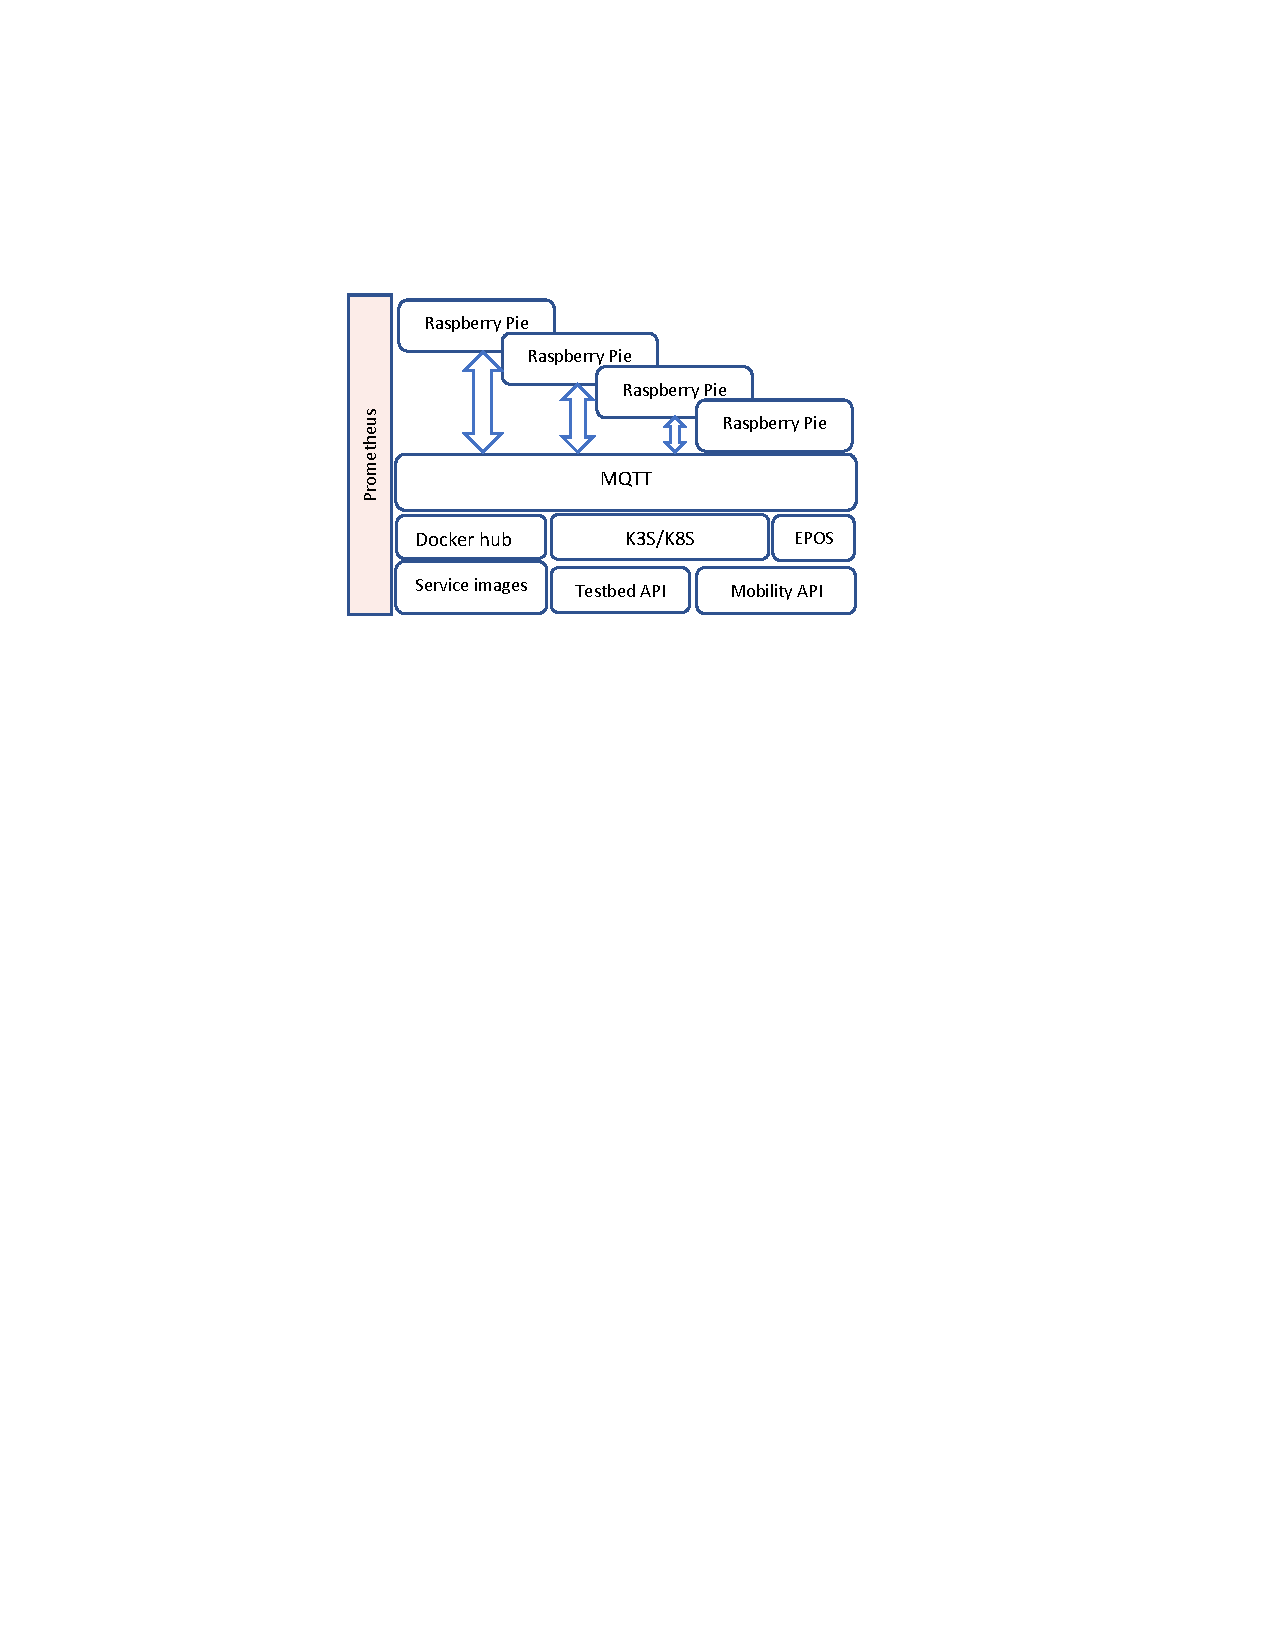
\includegraphics[clip, trim=5.7cm 17.5cm 6.9cm 5cm, width=\columnwidth]{figures/arch1.pdf}
\caption{Proposed test-bed architecture}
\label{fig:arch}
\end{figure}
%\fbox{
\subsection{V2I testbed API}
\par V2I API is the core component of the testbed. It implements the required functions and interfaces to create the infrastructure environment. The testbed API implements an abstraction for edge node that are necessary to build a network environment (topology definition and links creation). Furthermore, it allows the developer to apply resource models that
define the available resources for each host, and interact with the real components.
The real environment is built of raspberry pies and regular servers.... 
\par The testbed API interacts with kubernetes to instantiate the cluster nodes from raspberry pies and then instantiate V2I application components from pre-created Docker container images. A container image can be instantiated more than once in a network environment. An edge node is a collection of real nodes and their respective resources model and its associated access point to emulate a group of edge nodes. This abstraction allows the management of the related set of edge server and edge access points as a single entity. The V2X services could run in one or more nodes inside an edge environment.
\par The developed edge computing testbed API enables adding/removing agents and edge nodes, and connecting/disconnecting containers to agents dynamically within the created network topology. These extended features allow the emulation of real-world edge infrastructures in which it is possible to start and stop services instances at any point in time. Also, it allows the adjustment of the containers and the resource limitations (processing power and memory resources) at runtime by interacting with the kubernetes engine. 

\subsection{Kubernetes}
\subsection{MQTT}
\subsection{EPOS}
\subsection{Rasbpery pies}
Each edge node has a fixed position in a city that is the input provided by the developer.
The nodes positions could be extracted through the interaction with a real-world map offered by the interconnection with a mobility model that calculates the successive node position following the implemented mobility model. 
\subsection{SUMO}
\par The developed mobility API can be used to implement different mobility models. A real-world map, in our tests Munich city map, could be imported to the SUMO mobility simulator to model an accurate mobility model that simulates vehicle movements. 
\subsection{Services}
\par Deploying Services in the form of Docker instances offers a virtualized isolated environment for service execution at each host. The use of virtual interfaces and virtual links allows different nodes and instances to communicate easily.

\section{Application/scenario}\label{AA}
\par The workflow of creating and evaluating atypical V2I application using our testbed is demonestrated in the Fig.\ref{fig:workflow}.

\begin{figure*}
\fbox{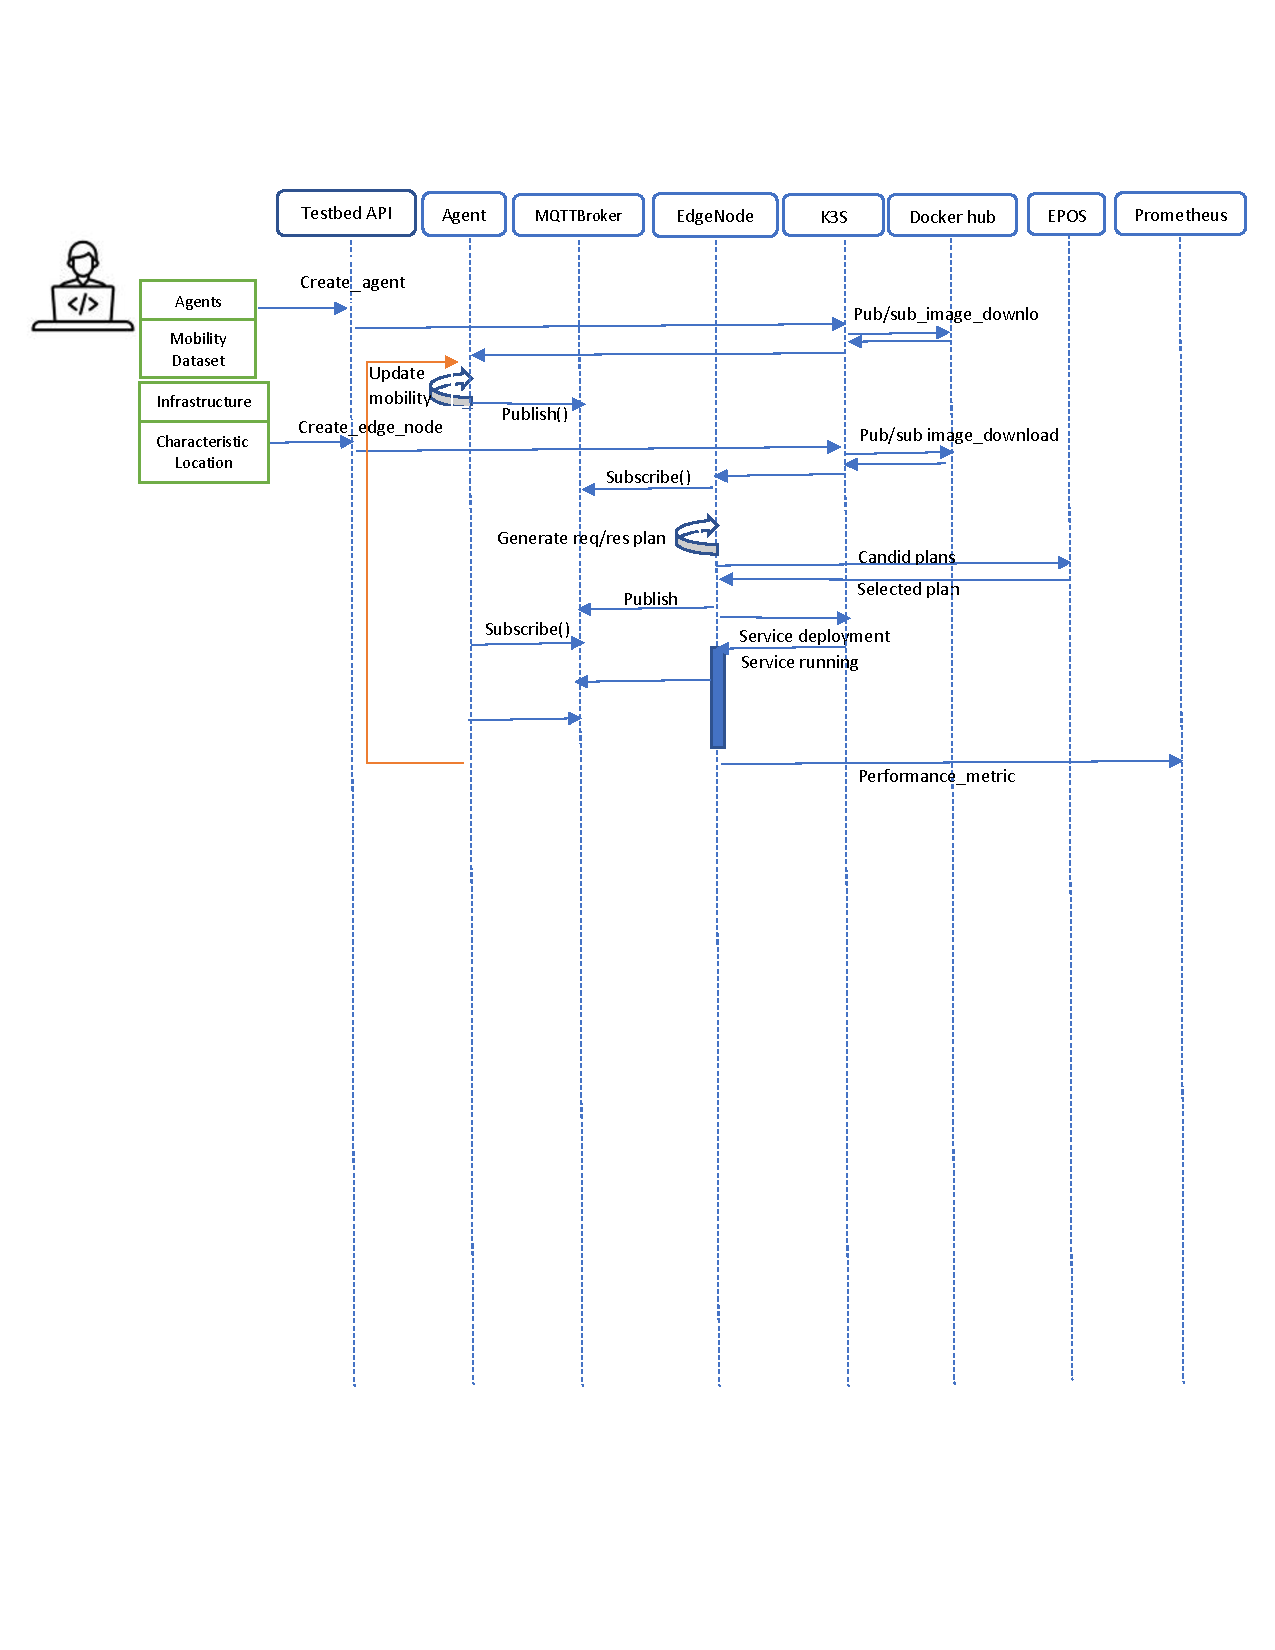
\includegraphics[clip, trim=0cm 13.3cm 0cm 3.2cm, width=\textwidth]{figures/workflow-1.pdf}}
\caption{V2I application workflow}
\label{fig:workflow}
\end{figure*}

\subsection{Methodology for evaluation}


\section{Evaluation}


\subsection{Threats to validity}


\subsection{Conclusion}

\section*{References}


\end{document}
